\chapter{Teoria dos Conjuntos}

Conjunto é uma coleção de elementos, não importando a ordem ou quantidade de vezes em que estes se apresentam. Qualquer coisa é um elemento em potencial. Se um elemento $x$ faz parte de um conjunto $A$, é dito $x \in A$. Se ele não faz parte, $x \not \in A$.

\begin{df}
Um conjunto é dito \emph{subconjunto} de outro se todos os elementos do primeiro pertencerem ao segundo. \[A \subset B \Leftrightarrow (\forall x) (x\in A \rightarrow x \in B)\].
\end{df}
\vspace{-24pt}
\begin{df}
Dois conjuntos são ditos \emph{iguais} se todos os elementos de um pertencerem ao outro e vice-versa.\[A=B \Leftrightarrow (\forall x)(x \in A \leftrightarrow x \in B)\]
\end{df}
\begin{df}
O número de elementos de um conjunto é chamado de \emph{cardinalidade} e é denotado por $|A|$.
\end{df}
\section{Representação de Conjuntos\cite{ticj}}
Conjuntos são usualmente denotados por letras latinas maiúsculas, enquanto seus elementos são normalmente denotados por letras latinas minúsculas ou por letras minúsculas munidas de índices numéricos. 

\subsection*{Extensão}
A forma mais simples de representar os elementos de um conjunto entre chaves, listando-os.
\begin{exemplo}
\[A=\{a_1,a_2,a_3,..., a_n\}\]
\end{exemplo}

\subsection*{Compreensão}
Podemos representar um conjunto especificando os seus elementos através de uma proposição. \begin{exemplo}
\[A=\{a_i | 0<i \le n\}\]
\end{exemplo}

\subsection*{Diagrama de Euler-Venn}
Podemos representar conjuntos através dos diagramas de Euler-Venn. Conjuntos finitos podem ser proveitosamente representados, por um plano determinado por uma linha fechada não entrelaçada inscrita em um quadrado ou retângulo. Nesse diagrama, os elementos do conjunto são representados por pontos internos ao recinto e elementos que não pertencem ao conjunto são representados por pontos externos. \par 
Um dos benefícios de representar conjuntos por meio de diagramas de Euler-Venn é a fácil visualização de subconjuntos, intersecções e outras regiões definidas nos conjuntos.
\begin{comment}
\begin{figure}[H]
  \caption{Diagrama de Euler-Venn}
  \centering
  \includegraphics[width=0.5\textwidth]{images/venn}
\end{figure}
\end{comment}

\section{Conjuntos Conhecidos}
Ao longo da nossa vida de estudante, somo expostos de maneira progressiva a conjuntos numéricos que se tornam, depois de um tempo, conhecidos. De início, temos os naturais, que também são conhecidos como números de contagem. Depois, se expandem para os Inteiros, que é quando somos apresentados aos números negativos.%colocar footnote sobre controversias nesta definição%. 
Na sequência temos os racionais e suas dizimas e frações, juntamente somos apresentados aos Irracionais. Para juntar todos estes números, unimos os conjuntos $\mathbb{Q}$ e $\mathbb{I}$ e obtemos os reais. Entretanto, observe a imagem abaixo:\\
%colocar uma imagem errada de conjuntos%
Se os reais podem ser definidos como a união dos conjuntos $\mathbb{Q}$ e $\mathbb{I}$, o que tem no espaço hashurado?
Por fim, temos os Complexos, que podem ou não ser trabalhados na educação básica, mas saiba você, aluno da graduação de matemática, que eles existem.

\subsection{Conjuntos Numéricos}
\subsubsection{$\mathbb{N}$ - Números Naturais}
Os números naturais são aqueles utilizados para contagem e ordenação. De forma ampla, os números naturais são uma propriedade de um conjunto: o conjunto $\{1,\alpha,4,a\}$ apresenta a propriedade $4$, pois possui quatro elementos. \[\mathbb{N}=\{0,1,2,3,4,5,\dots \}\]

\subsubsection{$\mathbb{Z}$ - Números Inteiros}
O conjunto dos números inteiros é formado pelos números naturais e seus opostos aditivos, constituindo um grupo com a operação adição definida. \[\mathbb{Z}=\{\dots, -3, -2, -1, 0, 1, 2, 3, \dots\}\]

\subsubsection{$\mathbb{Q}$ - Números Racionais}
O conjunto dos números racionais é derivado do conjunto dos números inteiros. Os números racionais são formados por frações de inteiros, representando partes de um inteiro. O conjunto $\mathbb{Q}$ é definido por \[\mathbb{Q}=\left\lbrace \frac{a}{b} \: | \: a,b \in \mathbb{Z}, b \neq 0 \right\rbrace\]

\subsubsection{$\mathbb{I}$ - Números Irracionais}
Os números irracionais são aqueles que não podem ser escritos como uma fração de inteiros (aqueles que não são racionais). Estes são constantes com infinitas casas decimais não-periódicas e raízes. São estes os números reais algébricos e transcendentes.
\subsubsection{$\mathbb{R}$ - Números Reais}
O conjunto dos números reais é definido por \[\mathbb{R}=\mathbb{Q} \cup \mathbb{I}\] e pode ser interpretado como todos os valores reais, como medidas.

\subsubsection{$\mathbb{C}$ - Números Complexos}
O conjunto dos números complexos é gerado a partir das raízes de índice par de números negativos. Os números são formados de uma parte real e uma parte imaginária - composta pela unidade $i$. O conjunto é definido como \[\mathbb{C}=\{a+bi \ | \ a,b \in \mathbb{R}, i^2=-1\}\]

\subsection{Conjunto Vazio}
O conjunto vazio, representado por $\emptyset$, é o conjunto que não possui elementos. Portanto, \[(\forall x)(x \in \emptyset) \: \Rightarrow \: F\]

\subsection*{Outros Conjuntos}
\begin{df}
O conjunto de todos os subconjuntos de $A$ é chamado de \emph{conjunto das partes}, conjunto potência ou apenas partes de $A$. É denotado por $\mathcal{P}(A)$ ou $2^A$. \begin{exemplo}
\[A=\{1, 2, 3\}\]
\[\mathcal{P}(A)=\{\emptyset, \{1\}, \{2\}, \{3\}, \{1,2\}, \{1,3\}, \{2,3\}, \{1,2,3\}\}\]
\end{exemplo}
O conjunto é denotado por $2^{A}$ pois possui exatamente $2^{|A|}$ elementos.
\end{df}
\begin{df}
Uma família de subconjuntos $\{A_i \: | \: i \in I\}$ de um conjunto $A$ é dita uma \emph{partição} de A se as seguintes propriedades são cumpridas:
\begin{itemize}
	\item $A_i \neq \emptyset, \forall i \in I$
	\item $\bigcup\limits_{i \in I} A_i = A$
	\item $A_i \cap A_j \neq \emptyset \Rightarrow A_i =A_j$
\end{itemize}
\end{df}

\section{Operações}
%texto, se quiser.
\subsection*{União}
O união de dois conjuntos resulta em um conjunto que possui os elementos de ambos os conjuntos.
\[A \cup B = \{x \: | \: x\in A \vee x \in B\}\]
\begin{figure}[H]
  \caption{União}
  \centering
  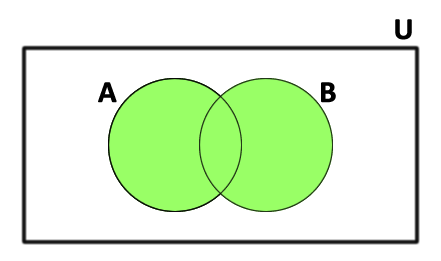
\includegraphics[width=0.5\textwidth]{algebra/imagens/uni}
\end{figure}

\subsection*{Intersecção}
A intersecção entre dois conjuntos é o subconjunto que possui os elementos que pertencem a ambos os conjuntos simultaneamente.
\[A \cap B = \{x \: | \: x\in A \wedge x \in B\}\]
\begin{figure}[H]
  \caption{Intersecção}
  \centering
  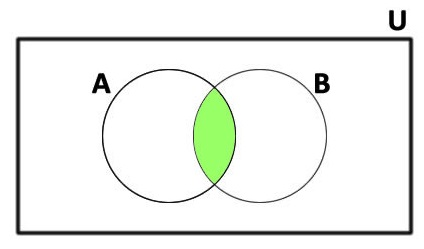
\includegraphics[width=0.5\textwidth]{algebra/imagens/intersect}
\end{figure}

\subsection*{Diferença}
A diferença entre $A$ e $B$ é o subconjunto que possui os elementos de $A$ que não são elementos de $B$.
\[A \smallsetminus B = \{x \: | \: x \in A \wedge x \not \in B\}\]
\begin{figure}[H]
  \caption{Diferença}
  \centering
  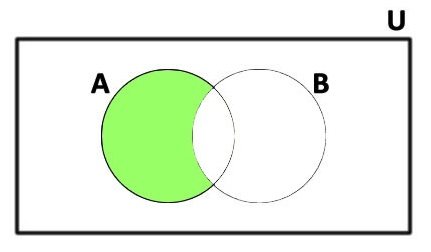
\includegraphics[width=0.5\textwidth]{algebra/imagens/diferen}
\end{figure}

\subsection*{Complementar}
O complementar de um conjunto $A$ é o conjunto de todos os elementos que não fazem parte de $A$.
\[A^{c}=\{x \: | \: x \not \in A\}\]
\begin{figure}[H]
  \caption{Complementar}
  \centering
  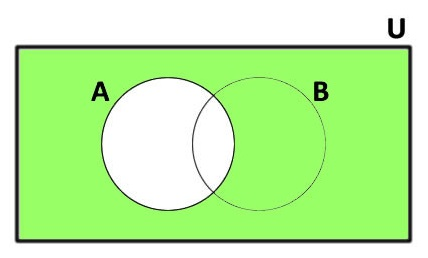
\includegraphics[width=0.5\textwidth]{algebra/imagens/comp}
\end{figure}

\subsection*{Diferença Simétrica}
A diferença simétrica $A \Delta B$ é o conjunto dos elementos que pertencem a apenas um dos conjuntos. Pode ser vista como a diferença entre a união e a intersecção $(A \cup B) - (A \cap B)$ ou como a união das diferenças $(A-B) \cup (B-A)$.
\[A \Delta B= \{x \: | \: x \in A \cup B \wedge x \not \in A \cap B\}\]
\begin{figure}[H]
  \caption{Diferença Simétrica}
  \centering
  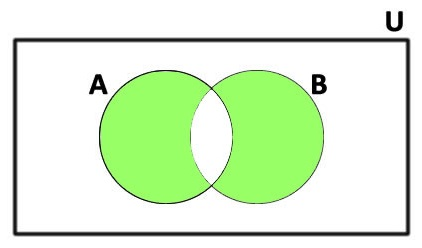
\includegraphics[width=0.5\textwidth]{algebra/imagens/difsim}
\end{figure}

\subsection*{Produto Cartesiano}
Originado apartir dos estudos de Descartes, que teve sua origem apartir da fundamentação da geometria analítica, o produto cartesiano (ou direto) é uma operação que relaciona  elementos de dois conjuntos em um elemento só.
\[A \times B = \{(x,y) \: | \: x \in A, y \in B\}\]